% Kompiuterijos katedros ir kibernetinio saugumo laboratorijos šablonas
% Template of Department of Computer Science II or cybersecurity laboratory
% Versija 1.3 2021 m. birželis [ March, 2015]

\documentclass[a4paper,12pt,fleqn]{article}
\usepackage[unicode,colorlinks=false]{hyperref}


\usepackage[utf8x]{inputenc}
%

\usepackage[L7x]{fontenc}
\usepackage{times}
\usepackage{ucs}
\usepackage{microtype}
\DisableLigatures{encoding = *, family = *}
 %package to switch the language
\usepackage{etoolbox}

  %set up of the page margins
\usepackage[top=2cm, bottom=2cm, left=3cm, right=1.5cm]{geometry}

 %1.1 line spacing
\linespread{1.1}


  %page numbering at the right side
\usepackage{fancyhdr}
\pagestyle{fancyplain}
\fancyhf{}
\renewcommand{\headrulewidth}{0pt} 
\fancyhfoffset[RO]{0cm}

  %to number at the bottom (exchange lines to number at the top)
\rfoot{\thepage}
  %\rhead{\thepage} %

% \usepackage[usenames,dvipsnames]{pstricks}
\urlstyle{same}
\hypersetup{
%  citecolor=Blue,
%  linkcolor=Blue,
%  urlcolor=Blue
pdfborder={0 0 0 }
}

 %for includegraphics
\usepackage{graphicx}



\usepackage[toc,page]{appendix}


\usepackage{caption}

 %for source codes
\usepackage{listings}
\lstset{commentstyle=\color{red},xleftmargin=10pt, framexleftmargin=6pt, numbersep=1mm, frame=single, numbers=left,numberstyle=\footnotesize,extendedchars=\true, inputencoding=utf8x,basicstyle=\footnotesize,extendedchars=true,
 keywordstyle=\color{black}\bfseries, breaklines=true, breakautoindent=true,framesep=8pt,linewidth=0.95\textwidth
}

 %for algorithms
\usepackage{algorithm}
\usepackage{algorithmic}
 %instead of the above two packages we can use algorithms2e
 %\usepackage[boxed,linesnumbered,vlined,slide]{algorithm2e}

 %special symbols
\usepackage{amsfonts}
\usepackage{amssymb}
\usepackage{amsmath}

 %for theorem like environments
\usepackage{amsthm}

 \usepackage{datetime}
 \renewcommand{\dateseparator}{--}


% SI system units
\usepackage{siunitx}
\sisetup{detect-all}
% Problem with fonts \SI{x.xx}{\micro\metre}, solved with updmap-sys --enable Map=utm.map
\renewcommand{\sfdefault}{uhv}
\renewcommand{\rmdefault}{utm}
\renewcommand{\ttdefault}{ucr}

% List management (itemize, etc.)
\usepackage{enumitem}

\newcommand*{\urlw}[1]{\href{#1}%
            {\nolinkurl{#1}}}

\numberwithin{equation}{section}


%%%%%%%%%%% lino įdėta
%
\usepackage{pifont,mdframed}

\newenvironment{warning}
  {\par\begin{mdframed}[linewidth=2pt,linecolor=red]%
    \begin{list}{}{\leftmargin=1cm
                   \labelwidth=\leftmargin}\item[\Large\ding{43}]}
  {\end{list}\end{mdframed}\par}
  

\newtoggle{inLithuanian}
 %If the report is in Lithuanian, it is set to true; otherwise, change to false
\settoggle{inLithuanian}{false}

%create file preface.tex for the preface text
%if preface is needed set to true
\newtoggle{needPreface}
\settoggle{needPreface}{false}

\newtoggle{signaturesOnTitlePage}
\settoggle{signaturesOnTitlePage}{true}


\theoremstyle{definition}
\newtheorem{definition}{\keyWordDefinition}
\newtheorem{example}{\keyWordExample}
\def\QED{\unskip\nobreak\hfill\kern5pt$\Box$}

\iftoggle{inLithuanian}{
%\usepackage[L7x]{fontenc}
\usepackage[english,lithuanian]{babel}

\newcommand{\todayiso}{\the\year \dateseparator \twodigit\month \dateseparator \twodigit\day}


\renewcommand{\today}{\number\year\space m. \space \ifcase\month\or
  sausio\or vasario\or kovo\or balandžio\or gegužės\or birželio\or
  liepos\or rugpjūčio\or rugsėjo\or spalio\or lapkričio\or
  gruodžio\fi
  \space\number\day\space d.}


 \usepackage{tocloft}
 \renewcommand\cftsecaftersnum{.} 
 \renewcommand\cftsubsecaftersnum{.} 
 \renewcommand\cftsubsubsecaftersnum{.}

 \usepackage{VUMIFKK}

 \DeclareCaptionLabelFormat{captionlt}{#2 #1}
   %smth is not fine with algorithms 
 \DeclareCaptionLabelFormat{captionltalg}{#2 #1 algoritmas}

 \usepackage{indentfirst}
 \renewcommand{\appendixtocname}{Priedai}
 \renewcommand{\appendixpagename}{Priedai}
 \renewcommand{\contentsname}{Turinys} 

 \renewcommand{\lstlistingname}{išeities kodas}
 \renewcommand{\figurename}{pav}
 \renewcommand{\tablename}{lentelė}


 \captionsetup*[lstlisting]{   
 labelsep=period,labelformat=captionlt
 }
 \captionsetup*[figure]{   
% labelsep=period,
 labelsep=space, %babel redefines pav to pav.
 labelformat=captionlt
 }
 \captionsetup*[table]{   
  labelsep=period,
  labelformat=captionlt
 }
 \renewcommand{\algorithmicrequire}{\textbf{Įvestis:}}
 \renewcommand{\algorithmicensure}{\textbf{Išvestis:}}

 \captionsetup*[algorithm]{   
 labelsep=period,labelformat=captionltalg
 }

\renewcommand{\thmhead}[3]{#2 #1#3}

}
{
%\usepackage[OT1,T1]{fontenc}
%\usepackage[L7x]{fontenc}



\usepackage[english]{babel}
\newcommand{\todayiso}{\twodigit\month \dateseparator \twodigit\day \dateseparator \the\year}
 \captionsetup*[algorithm]{   
 labelsep=period
 }
\captionsetup*[lstlisting]{   
 labelsep=period
 }
 \captionsetup*[figure]{   
 labelsep=period
 }
 \captionsetup*[table]{   
 labelsep=period
 }


}

%some kywords
 \def\keywordAbstract{\iftoggle{inLithuanian}{Santrauka}{Abstract}}
 \def\keywordAbstractOther{\iftoggle{inLithuanian}{Summary}{Santrauka}}
 \def\keyWordIntroduction{\iftoggle{inLithuanian}{Įvadas}{Introduction}}
 \def\keyWordConclusions{\iftoggle{inLithuanian}{Išvados ir rekomendacijos}{Conclusions and Recommendations}}

 \def\keyWordPreface{\iftoggle{inLithuanian}{Pratarmė}{Preface}}
 \def\keyWordAppendice{\iftoggle{inLithuanian}{Priedas}{Appendix}}
 \def\keyWordSignature{\iftoggle{inLithuanian}{parašas}{signature}}
 \def\keyWordDefinition{\iftoggle{inLithuanian}{apibrėžimas}{Definition}}
 \def\keyWordExample{\iftoggle{inLithuanian}{pavyzdys}{Example}}

\newcommand{\bothabstracts}[3]{
\setcounter{secnumdepth}{0}
\newpage
\hspace{2cm}
{\centering{\section{\keywordAbstract}}}

#1
\newpage
\hspace{2cm}
{\centering \section{\keywordAbstractOther}}

\begin{center}{\textbf{#2} }\end{center}

 #3
\setcounter{secnumdepth}{3}
}

 %non-numbered sections: #1 param: for labeling sec:#1, #2 -section title
\newcommand{\sectionWithoutNumber}[2]{\newpage
%\hspace{2cm}
\section*{#1}
\label{sec:#2}
\addcontentsline{toc}{section}{\nameref{sec:#2}}%{#3}
 }



\newcommand{\referenceSources}[1]{
\newpage
\cleardoublepage
\phantomsection
\iftoggle{inLithuanian}{
 \renewcommand{\refname}{Literatūros šaltiniai}

 \addcontentsline{toc}{section}{Literatūros šaltiniai}
 \markboth{\refname}{Literatūros šaltiniai}
 }
{

\addcontentsline{toc}{section}{References}
\markboth{References}{References}
}

\bibliographystyle{unsrt}
\bibliography{#1}
}



 \newcommand\authorsignature[1]{
\begin{flushright}
 \begin{minipage}[b]{0.45\textwidth}
  \centering
  \rule{\textwidth}{0.5pt}\\
   #1
  \end{minipage}
\end{flushright}
 }




 \newcommand\authorsignatures[5]{%
   \vspace{1cm}
   \authorsignature{#1}
   \ifstrequal{#2}{}{}{\vspace{0.3cm}
     \authorsignature{#2}
     \ifstrequal{#3}{}{}{\vspace{0.3cm}
      \authorsignature{#3}
      \ifstrequal{#4}{}{}{\vspace{0.3cm}
        \authorsignature{#4}
        \ifstrequal{#5}{}{}{\vspace{0.3cm}
         \authorsignature{#5}       
        }
      }
    }
} 
}

\newcommand{\authortitle}{
\iftoggle{signaturesOnTitlePage}{
\tiny{\keyWordSignature}
}{}
}

\newcommand{\depttitlepage}[8]
{
\thispagestyle{empty}
\begin{center}


\includegraphics[width=2cm]{jb_VU_zenklas}

%\vspace{-1cm}

\iftoggle{inLithuanian}
{ 
  VILNIAUS UNIVERSITETAS\\
  MATEMATIKOS IR INFORMATIKOS FAKULTETAS\\
  INFORMATIKOS INSTITUTAS\\
  KOMPIUTERIO IR DUOMENŲ MODELIAVIMO KATEDRA
}
{
  VILNIUS UNIVERSITY \\
  FACULTY OF MATHEMATICS AND INFORMATICS \\
  INSTITUTE OF COMPUTER SCIENCE\\
  <<DEPARTMENT OF COMPUTATIONAL AND DATA MODELING>> OR \\ <<CYBERSECURITY LABORATORY>>
}

\vspace{5cm}

#1\\
\vspace{0.5cm}
\textbf{\Large #2}
\end{center}

\vspace{5cm}


\hspace{0.5\textwidth}
\begin{minipage}{0.4\textwidth}
 \begin{flushleft} 
\iftoggle{inLithuanian}
{
 \ifstrequal{#3}{}{}{Atliko:\\[5pt]}
}
{
\ifstrequal{#3}{}{}{Done by:\\[5pt]}
}
%\noindent
\begin{tabular}{@{}lr}%\setlength\tabcolsep{0pt}
\ifstrequal{#3}{}{}{#3&\hspace{2cm}\authortitle\\[5pt]}
\ifstrequal{#4}{}{}{#4&\authortitle\\[5pt]}
\ifstrequal{#5}{}{}{#5&\authortitle\\[5pt]}
\ifstrequal{#6}{}{}{#6&\authortitle\\[5pt]}
\ifstrequal{#7}{}{}{#7&\authortitle\\}
\end{tabular}

\end{flushleft}

\end{minipage}

\vspace{0.5cm}
\hspace{0.5\textwidth}
\begin{minipage}{0.4\textwidth}
 \begin{flushleft} 

\ifstrequal{#8}{}{}
{

\iftoggle{inLithuanian}
{
Vadovas:
}
{
Supervisor:
}

#8

}

\end{flushleft}

\end{minipage}


\vfill

\begin{center}
Vilnius\\
\the\year
\end{center}

\iftoggle{needPreface}{
 \sectionWithoutNumber{\keyWordPreface}{preface}
Pratarmės (Preface) informacija


\iftoggle{inLithuanian}
{
\vspace{\baselineskip}\hfill
\today
}
{
 \vspace{\baselineskip}\hfill \today
}

 \vspace{5cm}

\iftoggle{signaturesOnTitlePage}{}
{
\authorsignatures{#3}{#4}{#5}{#6}{#7}
}
}{}
\newpage
}


\begin{document}
 % #1 -report type, #2 - title, #3-7 students, #8 - supervisor
 \depttitlepage{<<Super program name>> <<x>> year <<Report type>>}{Title in the primary language\\{\small Title in the secondary language}}{Name Surname} 
 {}{}{}{}% students 2-5
 {dr. Supervisor Name}

\tableofcontents


%keywords and notations if needed
\sectionWithoutNumber{Sutartinis terminų žodynas}{keywords}{Pateikiamas terminų sąrašas (jei reikia)}

 %both abstracts
\bothabstracts{Išmanieji telefonai tapo vienu iš dažniausiai naudojamų komunikacijos priemonių dėl jų geriausio ryšio, funkcionalumo ir produktyvumo. Nuolat tobulėjant išmaniųjų telefonų technologijoms, atsiranda naujų lygių pavojai. Didžioji rinkos dalis pasitiki „Android“ operacinės sistemos telefonais, kuri yra svarbi jėga konkurencinėje rinkoje, „Android“ ir „iOS“ duopolyje. „Android“ telefonai kaupia milžinišką duomenų kiekį, kurį galima saugoti tiek vietiniu, tiek nuotoliniu būdu, todėl teismo ekspertams jie suteikia patikimų duomenų, kurie yra labai svarbūs teismo ekspertizei. \\

Šiame darbe siekiama sukurti dinamišką įrankį, skirtą duomenų išgavimui, analizei ir parengimui teismo ekspertizei. Įrankis sukurtas atsižvelgiant į tai, jog dauguma esamų įrankių nėra suderinami su visais „Android“ mobiliaisiais įrenginiais. Įrankio programavimui buvo naudojama „Shell Script“ kalbą. Visos komandas buvo automatizuotis ir suskirstytos į skirtingus skriptus, kurie palengvina teismo ekspertizės analizę. Šis įrankis gali būti  paleistais „Linux“ ar „Windows“ (su „Windows Subsystem for Linux“) operacinėse sistemose. Norint išgauti duomenis, naudojama „ADB Shell“ komunikacija, naudojant root lygį, kuris pasiekiamas paleidus neoficialų atstatymo režimą. Tyrimo metu buvo atsižvelgta į skambučių žurnalo istoriją, SMS žinutes, naršyklės istoriją, nuotraukas ir kitus failus, kurie yra svarbūs teismo ekspertizei. Norint palengvinti tolimesnę duomenų analizę, jie yra suskirstomi į aplankus. \\

Darbo eigoje sukurta priemonė išgauna įrenginio duomenų particijos atvaizdą, jį išsaugo ir tinkamai suformatuoja išgautus duomenis taip, kad būtų patogu juos naudoti bylų sprendimui. Sukurtas įrankis veikia su dauguma „Samsung“ įrenginių, kurie neturi įjungto priverstinio šifravimo (angl. force encrypt) funkcijos. Jis taip pat gali būti pritaikytas duomenų ištraukimui iš kitų gamintojų įrenginių.}%tex-file of abstract in original language
{Darbo pavadinimas kita kalba} %if work is in LT this title should be in English
{Smartphones have become one of the most commonly used communication devices due to their improved connectivity, functionality, and productivity. As smart technologies continue to advance, new levels of potential risks emerge. The majority of the market relies on Android operating system phones, which holds a significant position in the competitive market, forming an Android-iOS duopoly. Android devices store a vast amount of data, which can be stored locally or remotely, providing forensic experts with reliable data that is crucial for forensic investigations.\\

The objective of this coursework is to develop a dynamic tool for data extraction, analysis, and preparation for forensic examination. The tool has been developed considering the fact that most existing tools are not compatible with all Android mobile devices. The tool has been programmed using the Shell Script language, utilizing commands that have been automated and divided into separate scripts, which facilitate forensic analysis. This tool can be used on Linux or Windows (with Windows Subsystem for Linux) operating systems. To access the data, ADB Shell communication is utilized on the root level, which can be achieved by booting into an unofficial recovery mode. During the development, considerations have been made for call log history, SMS messages, browser history, photos, and other files that are relevant to forensic examination. Data is organized into directories to facilitate further analysis.\\

The developed tool extracts the data partition image of the device, saves it, and properly formats the extracted data for convenient use in case resolution. This tool works with most Samsung devices that do not have the force encrypt feature enabled, and it can also be adapted for devices from other manufacturers.\\}%tex-file of abstract in other language


 %Introduction section: label is sec:intro
\sectionWithoutNumber{\keyWordIntroduction}{intro}
\textbf{Darbo aktualumas} Mobilieji telefonai per pastaruosius metus tapo populiarūs dėl savo didelio funkcionalumo, prieinamumo ir produktyvumo. Tačiau šios pažangios technologijos taip pat atnešė naujų iššūkių ir pavojų, ypač kriminalistikoje. Kriminalistinėje veikloje mobilieji įrenginiai tapo duomenų kaupimo ir komunikacijos priemonėmis, o juose sukaupti duomenys tapo svarbia medžiaga teisminėse ekspertizėse.\\

\textbf{Darbo problema} Duomenų tyrimai rankiniu būdu užima daug laiko bei yra mažiau tikslūs ir saugūs, nes daugumą procedūrų norint išgauti duomenis yra pasikartojančios ir galėtų būti automatizuotos naudojant skriptus, kurie automatiškai išgautų duomenis iš atvaizdo. Be to, pats atvaizdo sukūrimas sudaro galimybes efektyvesnei analizei, nes keli darbuotojai gali dirbti su tuo pačiu atvaizdu, pasidalinti darbais. Deja, dėl žymių skirtumų tarp skirtingų mobiliųjų telefonų modelių bei operacinės sistemos variacijų, labai sunku sukurti įrankį, kuris automatiškai tiktų kiekvienam telefonui, be jokių modifikacijų.
„Android“ operacinėje sistemoje su kiekvienu atnaujinimu, duomenų pasiekimo kelias gali būti ribojamas. Mobilieji telefonai su „Android“ operacine sistema vis dažniau vartojami, todėl dažnai tenka daryti jų teisminę ekspertizę. Sukurtas įrankis palengvintų darbuotojams duomenų išgavimo procesą. \\

\textbf{Darbo objektas.}  Prijungus telefoną, sukūrus jo disko atvaizdą, sumontavus (angl. mounted) jį bei išgavus ir apdorojus duomenis, tyrėjas galėtų atlikti daug kokybiškesnį bei greitesnį darbą, naudojant automatizuotą įrankį. Įrankio veikimo principas paprastas - kompiuteryje įrašytas įrankis prisijungia prie telefono, ištraukia atminties atvaizdą, pasiekia jame esančią informaciją, tvarkingai ją suformatuoja ir paruošia tolimesniam tyrimui. Įrankis turėtų  išgauti duomenis vientisa tvarką, nes bet koks vientisumo pažeidimas sunaikintų duomenų integralumą.\\

\textbf{Darbo tikslas.}  Darbo tikslas yra sukurti automatizuotą įrankį, kuris ištirtų „Android“ įrenginį ir palengvintų jo tyrimo procesą. Šis darbas aprašo, kaip galima atlikti mobilių telefonų, veikiančių su „Android“ operacine sistema, teisminę ekspertizę.\\

\textbf{Darbo uždaviniai: }
\begin{itemize}
 \setlength{\itemsep}{1pt}
  \setlength{\parskip}{0pt}
  \setlength{\parsep}{0pt}
    \item  Apžvelgti Android įrenginio architektūrą
    \item  Pademonstruoti veikimo modelį
    \item  Apžvelgti sukurto įrankio funkcionalumą
    \item  Aprašyti ateities planus tyrimui
\end{itemize}




 %the main part
\newpage
\section{Analysis}
\label{sec:motivation}
\subsection{some subection}
\label{sec:example}
Pateikiamas \ref{sec:example} poskyrio tekstas. Vienas iš šaltinių~\cite{KTZ}. Visas turinys priklauso \ref{sec:motivation} skyriui.

Example to cite~\cite{10.1145/3470451}

\subsubsection{The first sub-subsection}
\label{sec:data}
Pateikiamas trečio lygio poskyrio tekstas.

\begin{equation}
x = \sum_{i=1}^N m_i
\end{equation}

\begin{table}[!ht]\centering
\caption{Lentelė ... }
\label{tabl:table}
\begin{tabular}{l|r|}
test&test\\ \hline
test&test\\
\end{tabular}
\end{table}

Sprendimas pristatomas \ref{alg:1} algoritme, o įgyvendinimas -- \ref{abc} išeities kode.

\begin{algorithm}\caption{Algoritmas uždavinio sprendimui}
  \label{alg:1}
  \begin{algorithmic}
    \REQUIRE 
    \ENSURE 
\STATE a \AND b
\end{algorithmic}


\end{algorithm}



\begin{lstlisting}[caption={Pagrindinio metodo žingsniai},label={abc}]
public static void main(String args[]){
}
\end{lstlisting}

 %Conclusions section
\sectionWithoutNumber{\keyWordConclusions}{conclu}

Sukurtas įrankis, turi daug funkcionalumų. Gali automatiškai arba rankiniu būdu išgauti duomenis iš daugelio mobiliųjų įrenginių.  Įrankis tinkamas telefonams su ekrano užraktu bei be ekrano užrakto. Įrankis gali ištraukti duomenis iš „Android“ įrenginio „userdata“ particijos atvaizdo, bei gauti juos iš įrenginio, kuris jau paleistas „TWRP“ režime.  Darbo eigoje sukurtas įrankis gali taip pat ištraukti ir apdoroti SMS, kontaktų, skambučių, bei naršyklės duomenų bazes. Taip apdorota medžiaga gali būti panaudota teisminei ekspertizei. Skriptas turi daug informacinių dialogų, kurie leidžia vartotojui lengvai suprasti kas vyksta ir kokius žingsnius reikia įvykdyti, kad duomenų išgavimas vyktų sklandžiai.

Įrankis veikia su daugeliu Samsung įrenginių, bei su kitais įrenginiais, kuriems turime galimybę suteikti „root“ teises arba įrašyti neoficialų atstatymo režimą. 

Darbo metu atliktame tyrime panaudotas įrankis sėkmingai ištraukia duomenis iš „Samsung Galaxy S5“ (veikiančio su naujausia jam prieinama „Android 6.0.1“ versiją) bei  „Samsung Galaxy S3 NEO“ (veikiančiu su naujausia jam prieinama „Android 4.4.4“ versiją). Iš šių mobiliūjų įrenginių pavyko išgauti visus analizei vertingus failus, o prireikus, tolimesnei analizei, įrankis suteikia galimybę sumontuoti atvaizdą ir atlikti analizę rankiniu būdu, analizuojant kitų programėlių duomenų bazes. 

Įrankis ne tik išgauna duomenis, bet ir juos tinkamai suformatuoja, į lengvai skaitomus tekstinius failus. Šis funkcionalumas leidžia žmonėms kurie niekada nedirbo su duomenų bazių analize lengvai peržiūrėti duomenis, tokius kaip SMS žinutes sudėliotas chronologiškai pagal gavėją, naršomų internetinių puslapių istoriją su naršymo datomis, bei URL adresais. 

Kadangi tai tik pirma pabaigta įrankio versija, jo automatinė duomenų išgavimo procedūra ribota veikti su Samsung įrenginiais. Atsižvelgiant į tai jog Lietuvoje pirmauja Samsung gamybos įrenginiai, sukurtas įrankis gali būti vertingas teisminėms analizėms. Remiantis Statcounter statistika \cite{StatcounterLithuania} (14 pav.),  virš trečdalis Lietuvoje naudojamų įrenginių yra Samsung gamybos.
\begin{figure} [h]
    \centering
    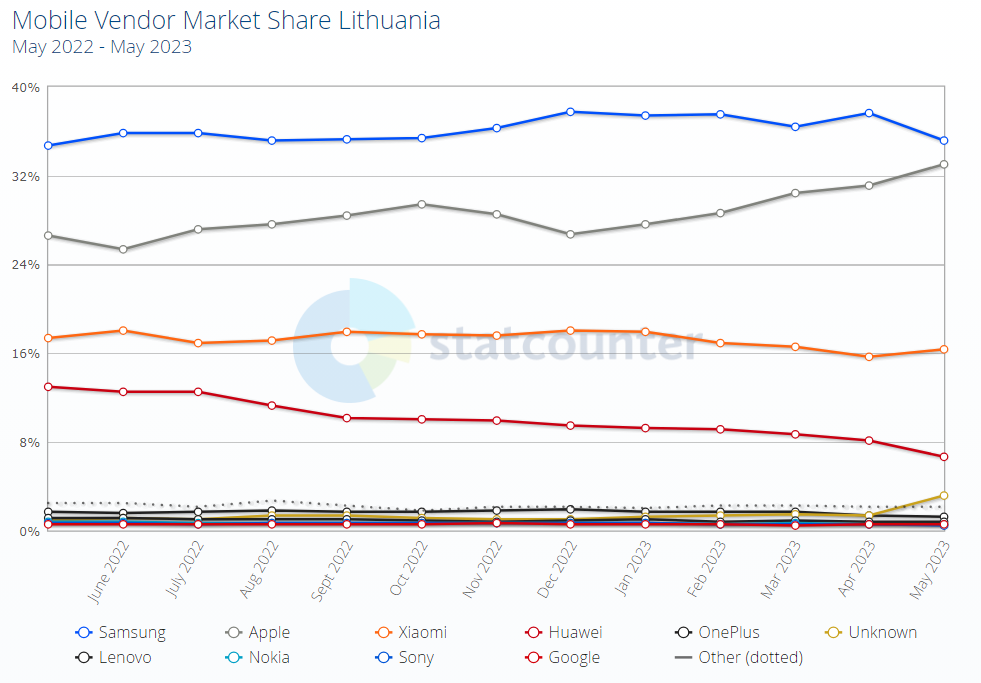
\includegraphics[width=0.85\linewidth]{stat_lt2.png}
    \caption{Mobiliųjų įrenginių pasiskirstymas pagal gamintojus Lietuvoje}
    \label{fig:LT_tel_statistics}
\end{figure}

%ateities darbų gairės, planas/next steps of the work
\sectionWithoutNumber{Ateities tyrimų planas}{future}{Pristatomi ateities darbai ir/ar jų planas, gairės tolimesniems darbams....}


 %file literatureSources.bib
\referenceSources{literatureSources}



%% this part is optional
\newpage
\begin{appendices}
Dokumentą sudaro du priedai: \ref{app:a} priede  ....
\newpage
\section{Pirmojo priedo pavadinimas}
\label{app:a}
Pirmojo priedo tekstas ...

\newpage
\section{Antrojo priedo pavadinimas}
Antrojo priedo tekstas ...

\end{appendices}


\end{document}
